\documentclass[norsk]{article}
\usepackage[norsk]{babel}
\usepackage{parskip}
\usepackage[utf8]{inputenc}
\usepackage{graphicx}
\usepackage{float}

\renewcommand{\thesubsection}{\thesection.\alph{subsection}}
\author{David Kolden, davidko}

\title{UNIK 4490 - Obligatorisk oppgave 1}
\begin{document}
\maketitle
\section{Øvelse 1}

\subsection{ }
Finner poler ved å løse \(s(1 + T_Ms) = 0\) som gir polene \(s = 0\) og \(s = -\frac{1}{T_M}\). Systemet er stabilt for alle positive verdier av \(T_M\).

\subsection{ }
Figur 1 viser blokkskjema for \(\frac{X(s)}{U(s)} = H(s) = \frac{1}{s(1 + T_Ms)}\)
\begin{figure}[!htb]
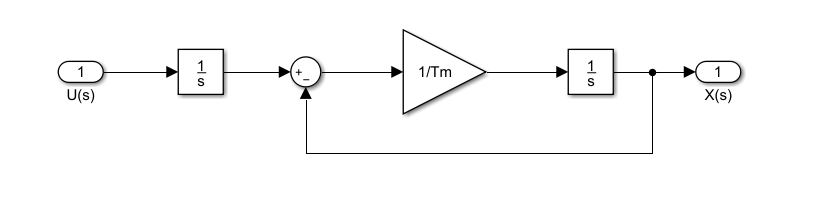
\includegraphics[height=3.5cm]{illustrations/oppg1b_illu}
\caption{Blokkskjema for \(H(s)\)}
\end{figure}

\subsection{ }
\(H(s)\) har to poler og er derfor et andreordens system.

Setter \(U(s) = K(1 + T_Ds)E(s)\), \(E(s) = R(s) - X(s)\), \(U(s) = K(1 + T_Ds)(R(s) - X(s))\) sammen med \(H(s)\):
\[X(s) = H(s)U(s) = H(s)K(1+T_Ds)(R(s) - X(s))\] 
\[X(s) = H(s)K(1+T_Ds)R(s) - H(s)K(1+T_Ds)X(s)\]
\[X(s)(1 + H(s)K(1+T_Ds)) = H(s)K(1+T_Ds)R(s)\]
\[\frac{X(s)}{R(s)} = H_C(s) = \frac{H(s)K(1+T_Ds)}{1+H(s)K(1+T_Ds)}\]
\[H_C(s) = \frac{K(1+T_Ds)}{\frac{1}{H(s)} + K(1+T_Ds)}\]

Setter inn for \(H(s)\):
\[H_C(s) = \frac{K(1+T_Ds)}{s(1+T_Ms)+ K(1+T_Ds)}\]
\[H_C(s) = \frac{K(1+T_Ds)}{s^2T_M + s + KT_Ds + K}\]
\[H_C(s) = \frac{(1+T_Ds)}{s^2\frac{T_M}{K} + s(\frac{1}{K}+T_D) + 1}\]

Ser at systemet med kontroller fortsatt er et andreordens system.
\subsection{ }
Figur to viser blokkskjema for systemet med kontroller (\(H_C(s)\))
\begin{figure}[!htb]
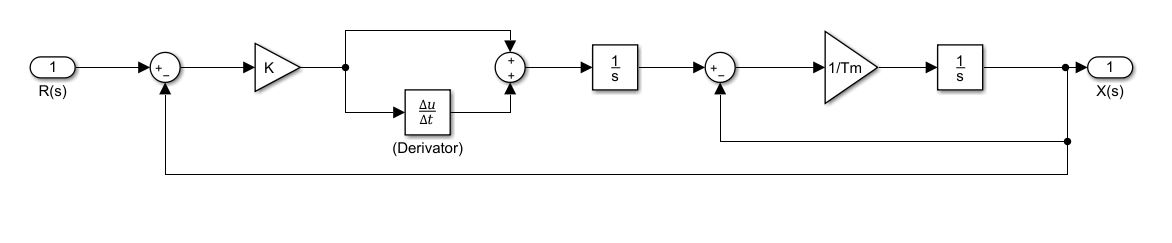
\includegraphics[height=2.9cm]{illustrations/oppg1d_illu}
\caption{Blokkskjema for \(H_C(s)\)}
\end{figure}

\subsection{ }
\(H_C(s)\) har ett nullpunkt og to poler. Nullpunktet finnes ved å sette telleren i \(H_C(s)\) til null, mens man finner polene ved å sette nevneren til null. Polene kan dermed finnes med uttrykket
\[s = \frac{-(\frac{1}{K} + T_D) \pm \sqrt{(\frac{1}{K} + T_D)^2 - 4\frac{T_M}{K}}}{2\frac{T_M}{K}}\]

mens nullpunktene finnes med uttrykket
\[s = -\frac{1}{T_D}\]

Ved å sette inn for \(T_M = 2\) og \(T_D = 1\) får vi til slutt et nullpunkt i \(s = -1\) og to poler i
\[s = \frac{-(\frac{1}{K} + 1) \pm \sqrt{(\frac{1}{K} + 1)^2 - 4\frac{2}{K}}}{2\frac{2}{K}}\]

Locusplot:
\begin{figure}[!htb]
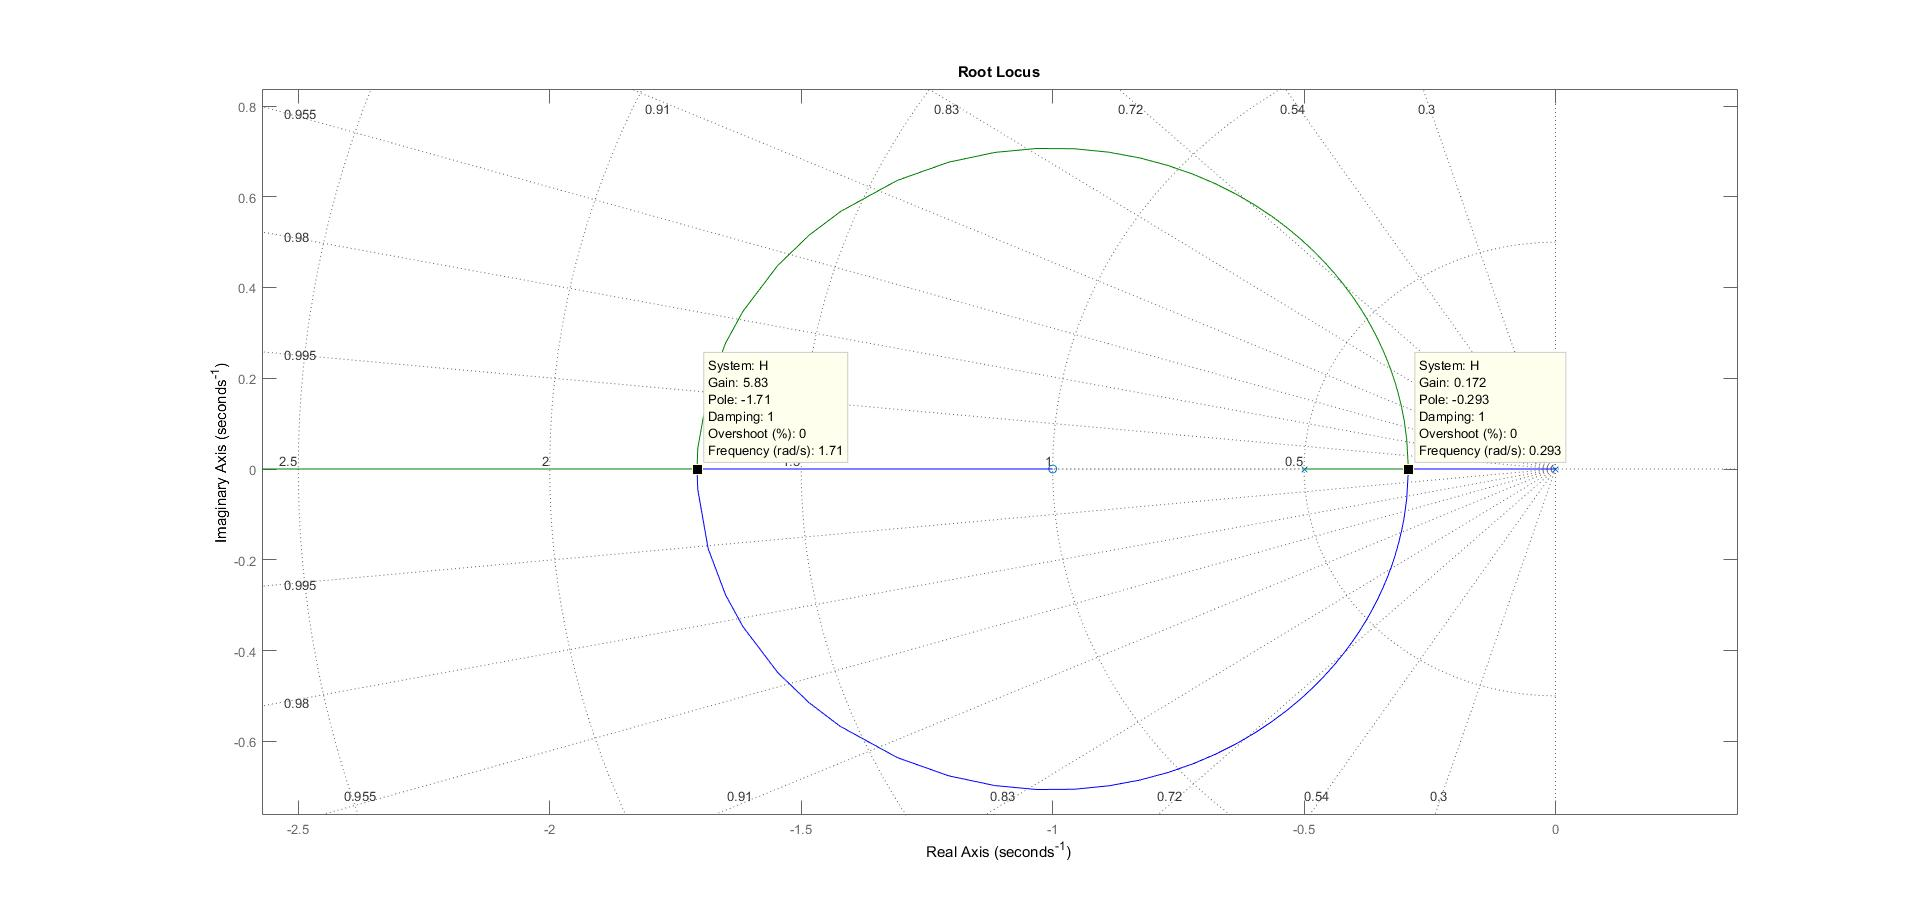
\includegraphics[height=10cm]{illustrations/oppg1e_illu}
\caption{Locusplot av \(H_C\)}
\end{figure}

\section{Øvelse 2}

\section{Øvelse 3}
\subsection{ }
\subsection{ }
\subsection{ }
\subsection{ }
\subsection{ }
\subsection{ }
\subsection{ }
\subsection{ }
\end{document}